\subsubsection{Kürzester Weg finden}

Da es nur 8 Knoten im Graph gibt, wurde von Anfang an vermutet, dass die Geschwindigkeit des Algorithmus vernachlässigt werden kann.

Um zu überprüfen, dass diese These stimmt, wurde ein traditioneller Dijkstra Algorithmus in Python implementiert. Dabei wurde von einem Knoten den kürzesten Weg zu allen anderen Knoten im vorgegebenen Graphen berechnet. währenddessen wurde die Zeit für die Berechnungen gestoppt. Um Hardware Einflüsse zu minimieren, wurde dieses Skript auch auf einem Single-Board Computer, namentlich einem Raspberry Pi 4 (4GB) ausgeführt, und einige male wiederholt. Was uns zu nachfolgender Ausgabe und Kenntnissen bringt:

\begin{figure}[H]
\begin{subfigure}{0.275\textwidth}
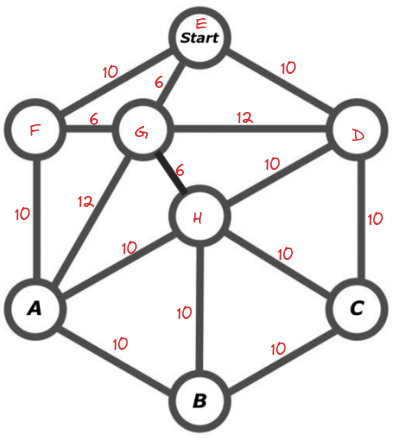
\includegraphics[width=0.95\linewidth]{img/graph_with_weighted_edges.png} 
\caption{Gewichteter Graph}
\label{fig:weighted-graph}
\end{subfigure}
\begin{subfigure}{0.720\textwidth}
\begin{footnotesize}
\begin{verbatim}
Shortest distance from E to A is 18 via path: E -> G -> A
Shortest distance from E to B is 22 via path: E -> G -> H -> B
Shortest distance from E to C is 20 via path: E -> D -> C
Shortest distance from E to D is 10 via path: E -> D
Shortest distance from E to E is 0 via path: E
Shortest distance from E to F is 10 via path: E -> F
Shortest distance from E to G is 6 via path: E -> G
Shortest distance from E to H is 12 via path: E -> G -> H
This calculation took about 0.128ms
\end{verbatim}
\end{footnotesize}
\caption{Skript Ausgabe}
\label{fig:djikstra-test-skript-output}
\end{subfigure}

\caption{Djikstra Algoritmus Test mit Python}
\label{fig:djikstra-test-output}
\end{figure}

Um den kürzesten Pfad achtmal zu berechnen, wurden etwa 0,128 ms benötigt, was ausreichend schnell ist. Aufgrund dieses Tests wurde entschieden, einen selbst implementierten, einfachen Dijkstra-Algorithmus zu verwenden, da es wichtig ist, dass der Algorithmus möglichst leichtgewichtig ist, da nur begrenzte Rechenleistung und Speicher zur Verfügung stehen.

Das Skript wurde in einem Github Gist veröffentlicht und ist unter folgendem Link aufrufbar: \url{https://gist.github.com/dimschlukas/2632116f913b1e10eea9be40e62b2630}

\subsubsection{Kamera Position}\label{camera-position}

Die Platzierung der Kamera ist ein entscheidender Faktor, um sicherzustellen, dass sie die gewünschten Objekte und Bereiche korrekt erfassen kann. Im Folgenden werden die relevanten Parameter erläutert:

\begin{itemize}
    \item Kamera wird auf einer Höhe von 22.5cm montiert.
    \item Field of View der Kamera beträgt 66 Grad.
    \item Kamera soll Knoten in einer nähe bis zu 15cm vor dem Roboter aufzeichnen.
    \item Kamera soll Objekte bis zu 2 Meter Entfernung aufzeichnen.
\end{itemize}

Nachfolgend skizziert wie diese Parameter die Position und Neigung der Kamera definieren:

\begin{figure}[H]
    \centering
    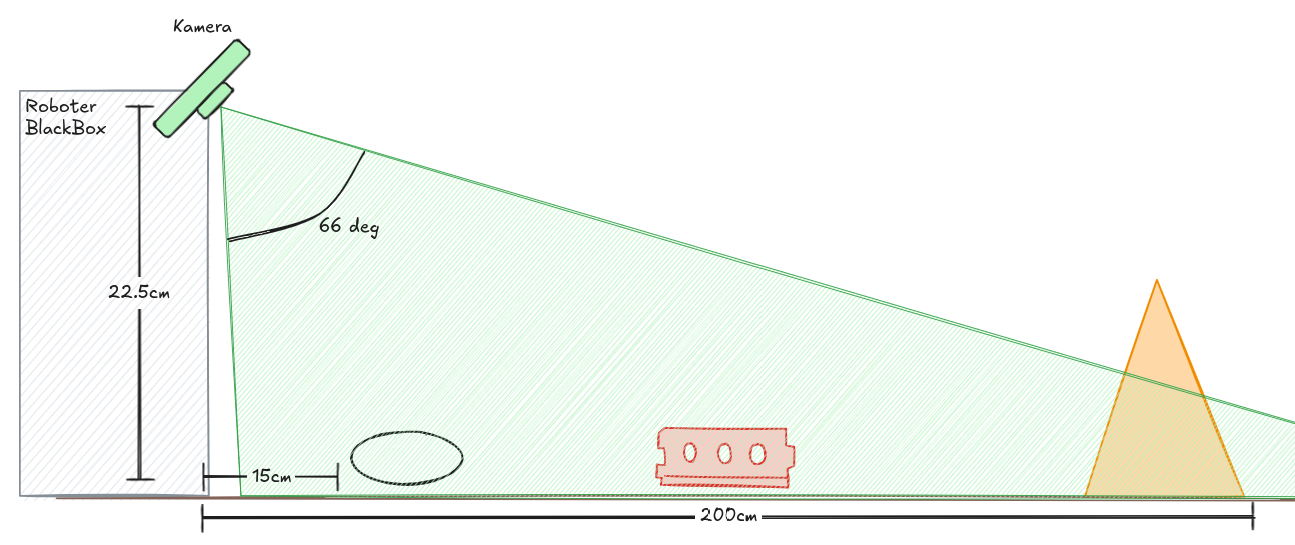
\includegraphics[width=1\linewidth]{assets/informatik-prototyp/camera/camera_position.png}
    \caption{Skizze der Kamera Positionierung}
    \label{fig:camera-position}
\end{figure}

Aus den Parametern kann also berechnet werden, dass die Kamera in einem Winkel von ca. 56 Grad eingebaut werden muss. Um die Knoten in der nähe sowie die Pylonen in der Distanz zu erfassen:

Nachfolgend dies dargestellt in einem Graphen mit korrekten Proportionen:

\begin{figure}[H]
    \centering
    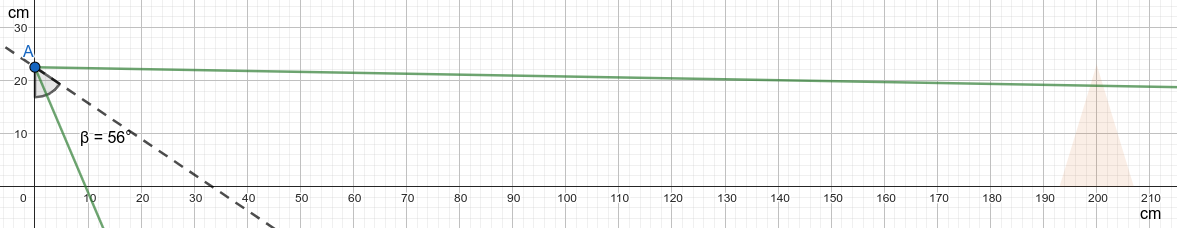
\includegraphics[width=1\linewidth]{assets/informatik-prototyp/camera/camera_position_exact_bigger.png}
    \caption{Graph der Kamera Positionierung}
    \label{fig:camera-position-exact}
\end{figure}





\subsubsection{Winkelerkennung}\label{winkelerkennung}

Um die Winkel der abgehenden Kanten eines Knoten zu detektieren, macht unser Roboter vor dem Befahren eines Knotens ein Bild dessen. Dazu ist jedoch zu beachten, wie in Kapitel \ref{camera-position} beschrieben, wird unsere Kamera in einem Winkel von 56 Grad montiert. So können wir naheliegende Knoten vor dem Roboter, wie auch weit entfernte Pylonen in einem Bild erkennen, ohne die Kamera schwenken zu müssen.
Da wir dadurch nun aber verzerrte Bilder aufzeichnen, muss an dem Bild zuerst eine geometrische Transformation durchgeführt werden. Sodass wir schlussendlich ein verzerrungsfreihe Ansicht auf den Knoten haben. Anschliessend können die einzelnen Winkel ohne Probleme durch maskieren und detektieren von Formen mittels Opencv berechnet werden.

Nachfolgend wird dies Schritt für Schritt nachvollziehbar dargestellt:

\begin{enumerate}
    \item Vor dem Knoten anhalten und Bild aufnehmen
    \begin{figure}[H]
        \centering
        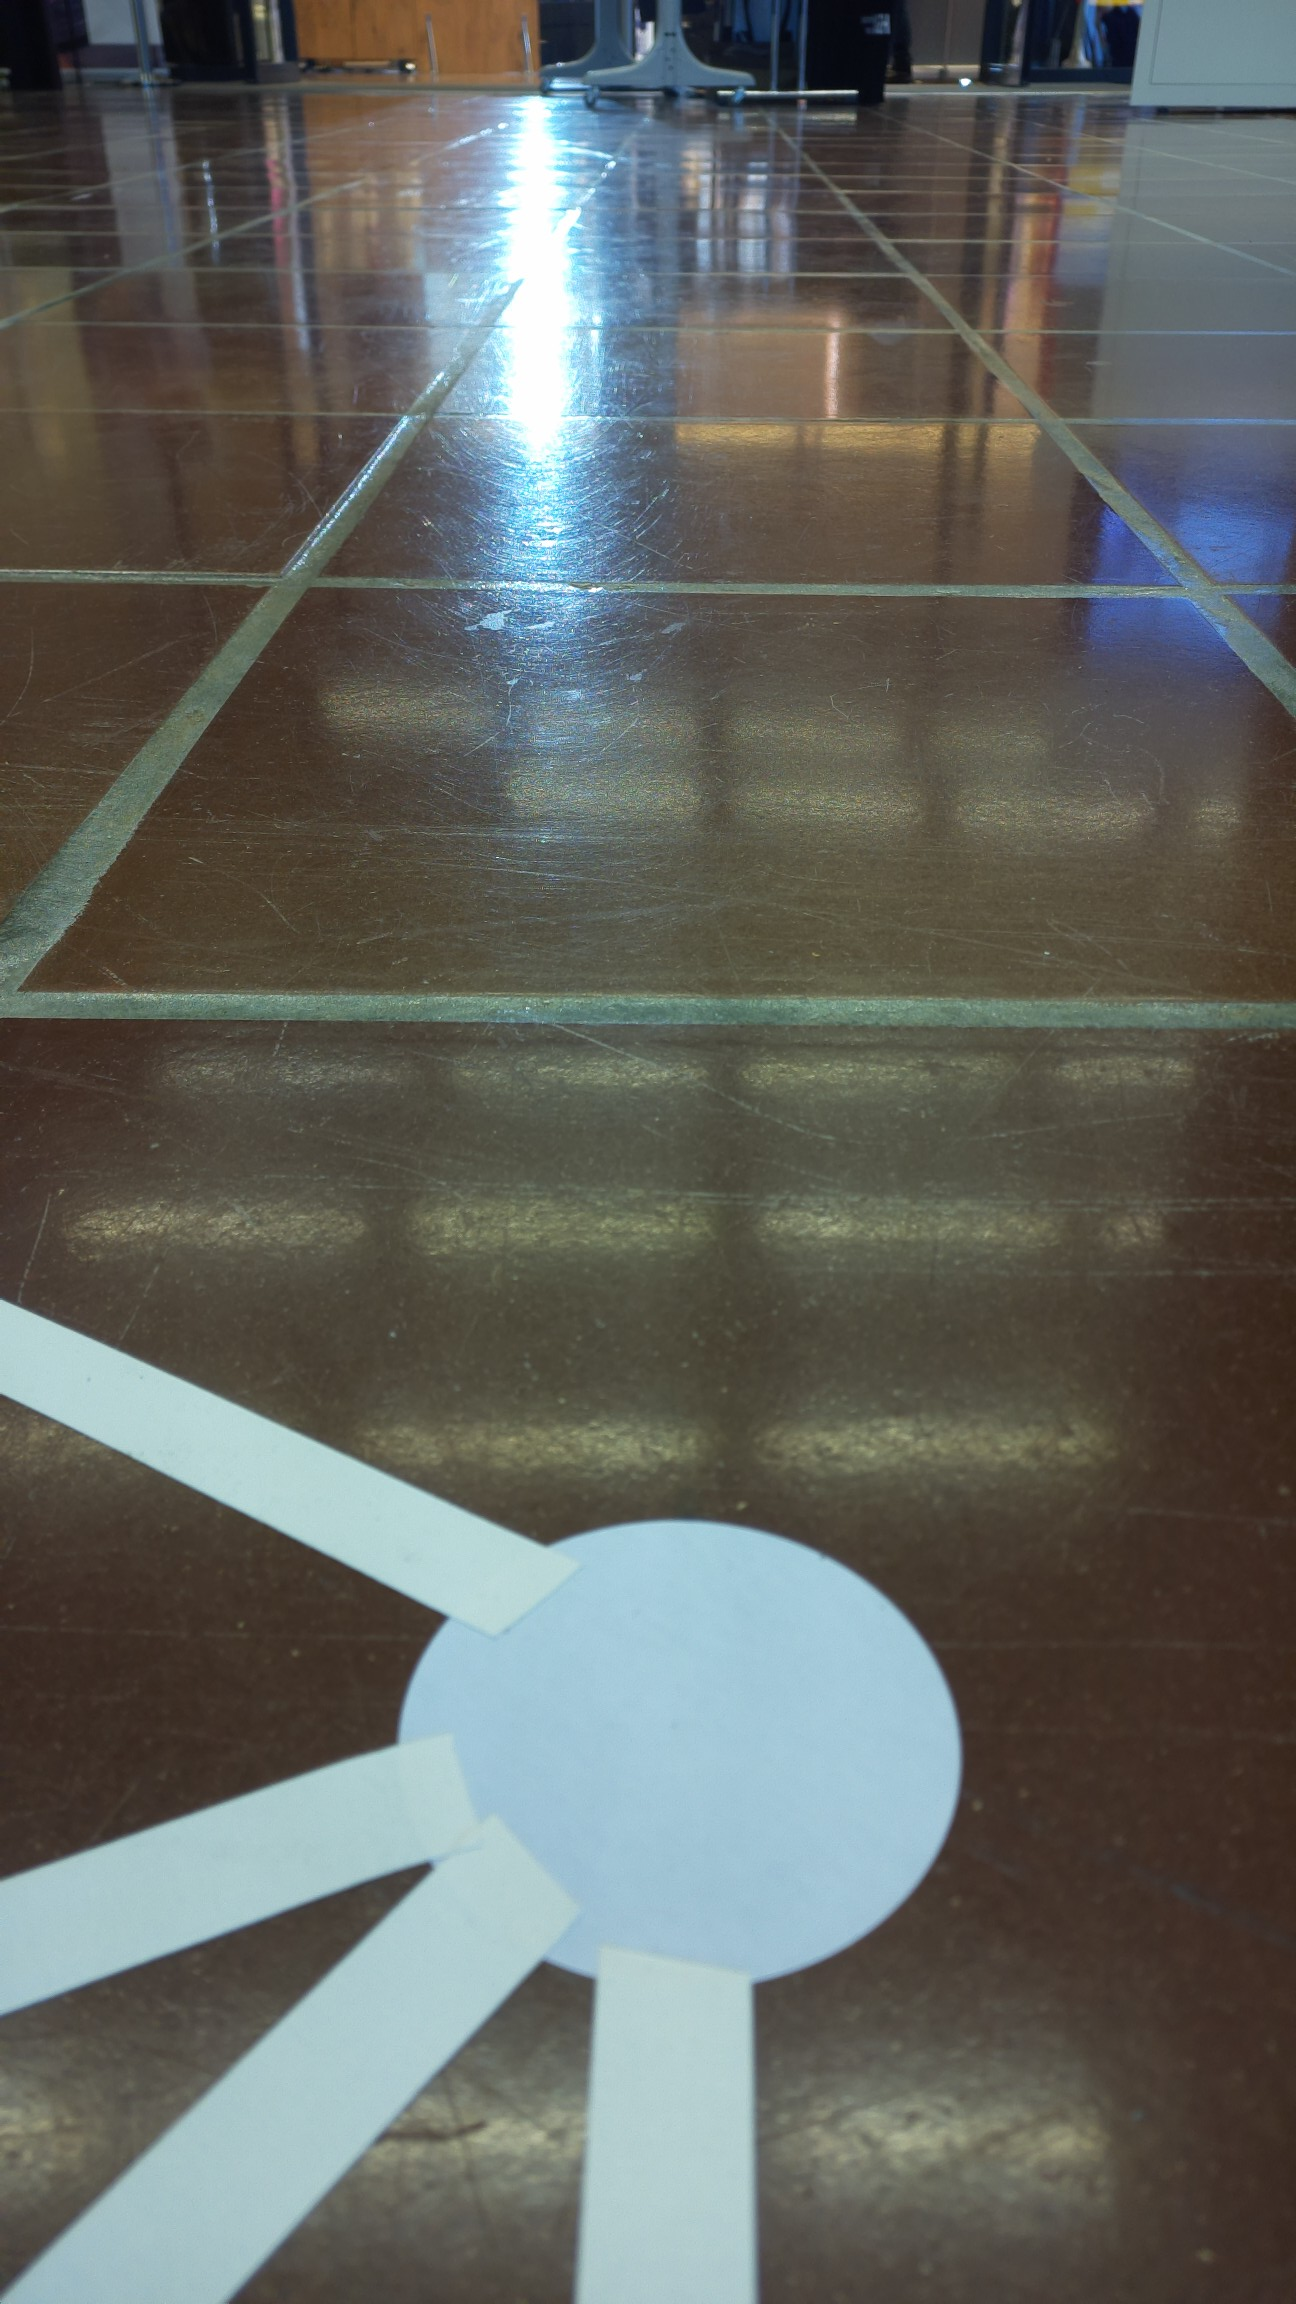
\includegraphics[width=0.5\linewidth, angle=90]{assets/informatik-prototyp/opencv/angle_detection/image_taken_by_pi_camer_before_node.jpg}
        \caption{Originale Kamera Aufnahme eines Knotens}
        \label{fig:before-node}
    \end{figure}
    \item Geometrische Transformation anhand fix definierten Punkten anwenden
        \begin{figure}[H]
        \centering
        \begin{subfigure}{0.4\textwidth}
        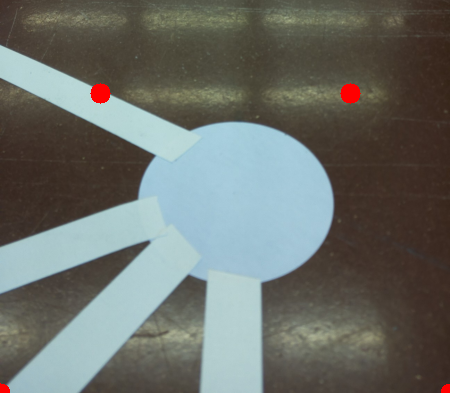
\includegraphics[width=0.95\linewidth]{assets/informatik-prototyp/opencv/angle_detection/node_before_transformation_corners.png} 
        \caption{Vier Punkte für Transformation}
        \label{fig:node-before-geometric-transform}
        \end{subfigure}
        \begin{subfigure}{0.4\textwidth}
        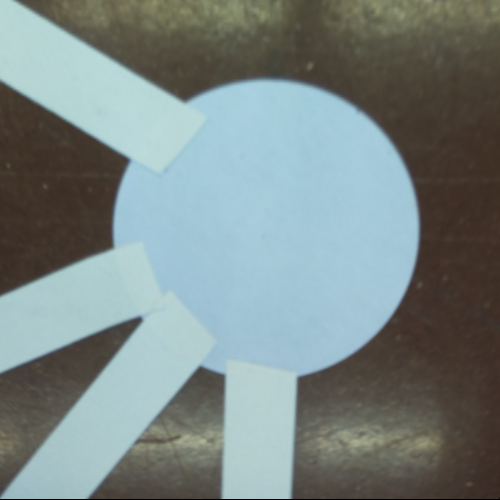
\includegraphics[width=0.95\linewidth]{assets/informatik-prototyp/opencv/angle_detection/node_after_transformation.png} 
        \caption{Nach Transformation}
        \label{fig:node-after-geometric-transform}
        \end{subfigure}
        \caption{Geometrische Transformation}
        \label{fig:node-geometric-transform}
        \end{figure}
    \item Knoten maskieren und dessen Mittelpunkt detektieren
        \begin{figure}[H]
        \centering
        \begin{subfigure}{0.4\textwidth}
        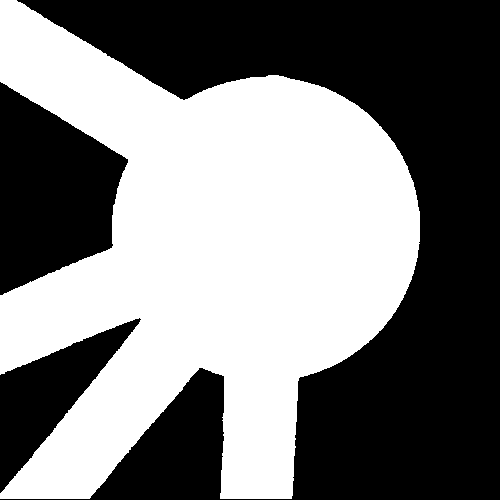
\includegraphics[width=0.95\linewidth]{assets/informatik-prototyp/opencv/angle_detection/node_after_transformation_masked.png} 
        \caption{Maskieren}
        \label{fig:node-masked}
        \end{subfigure}
        \begin{subfigure}{0.4\textwidth}
        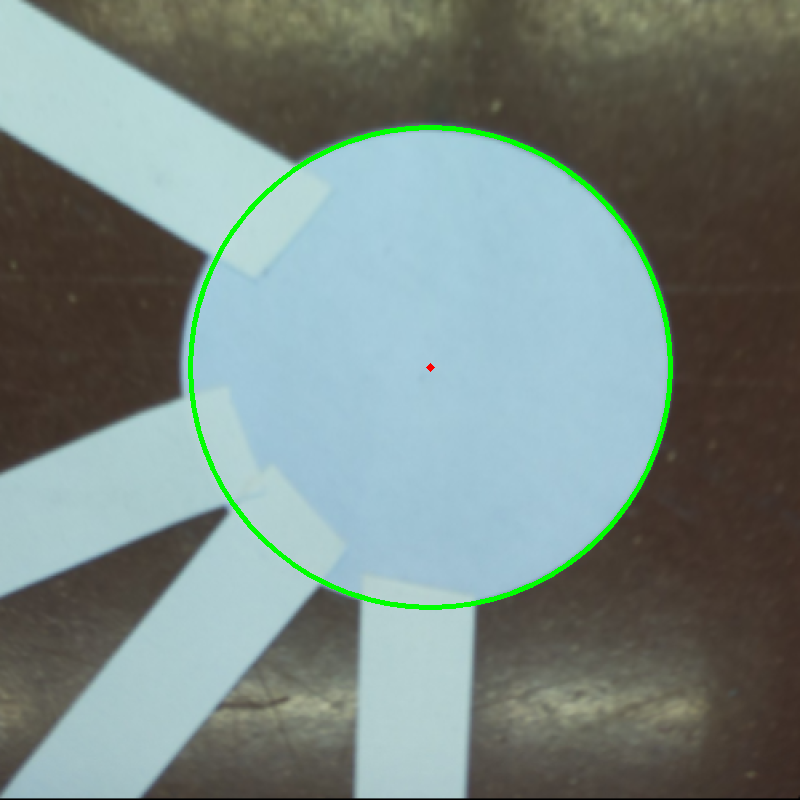
\includegraphics[width=0.95\linewidth]{assets/informatik-prototyp/opencv/angle_detection/node_detecting_center.png} 
        \caption{Mittelpunkt des Knoten detektieren}
        \label{fig:node-center}
        \end{subfigure}
        \caption{Knoten und dessen Mittelpunkt detektieren}
        \label{fig:detecting-node}
        \end{figure}
    \item Ausgehende Kanten maskieren
        \begin{figure}[H]
        \centering
        \begin{subfigure}{0.4\textwidth}
        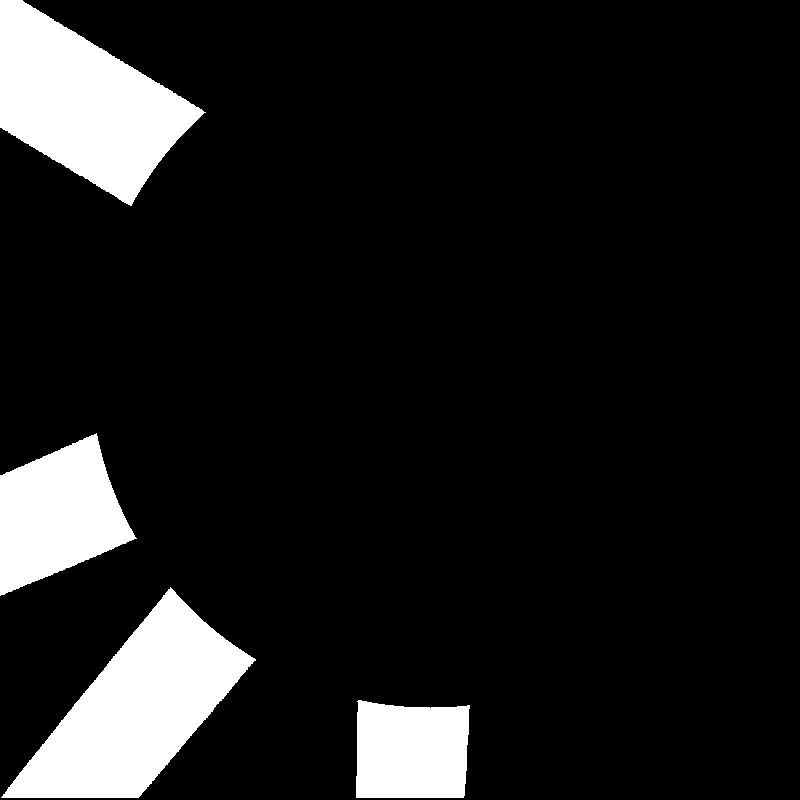
\includegraphics[width=0.95\linewidth]{assets/informatik-prototyp/opencv/angle_detection/edge_masked.png} 
        \caption{Nur Kanten maskieren}
        \label{fig:edge-masked}
        \end{subfigure}
        \begin{subfigure}{0.4\textwidth}
        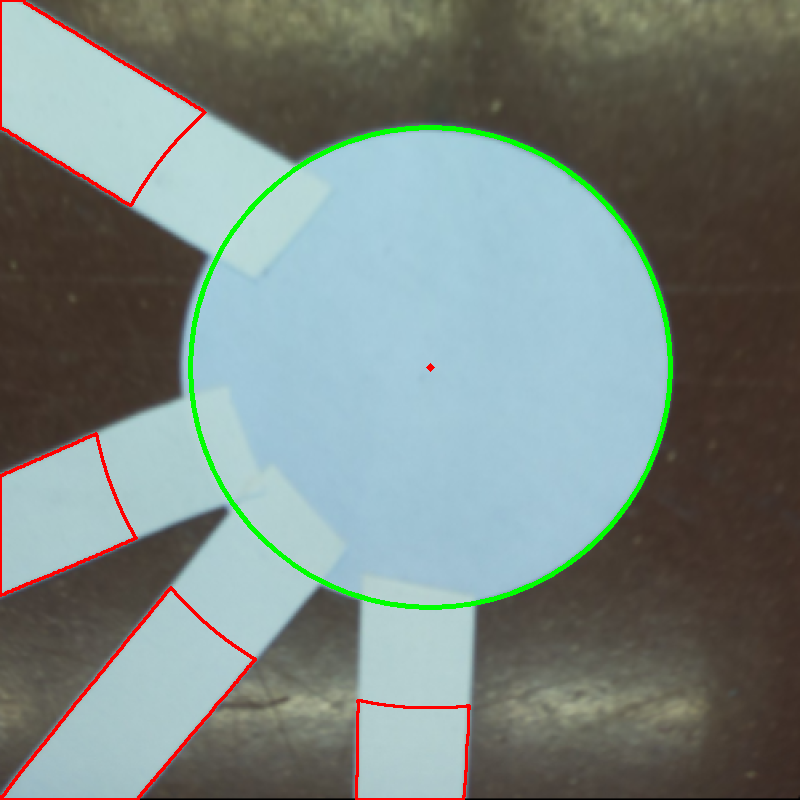
\includegraphics[width=0.95\linewidth]{assets/informatik-prototyp/opencv/angle_detection/edge_contours.png} 
        \caption{Kontur der Kanten zeichnen}
        \label{fig:edge-contours}
        \end{subfigure}
        \caption{Kanten detektieren}
        \label{fig:detecting-edges}
        \end{figure}
    \item Geometrischer Schwerpunkt der Kanten berechnen und Winkel zu Knoten Zentrum berechnen.
        \begin{figure}[H]
        \centering
        \begin{subfigure}{0.4\textwidth}
        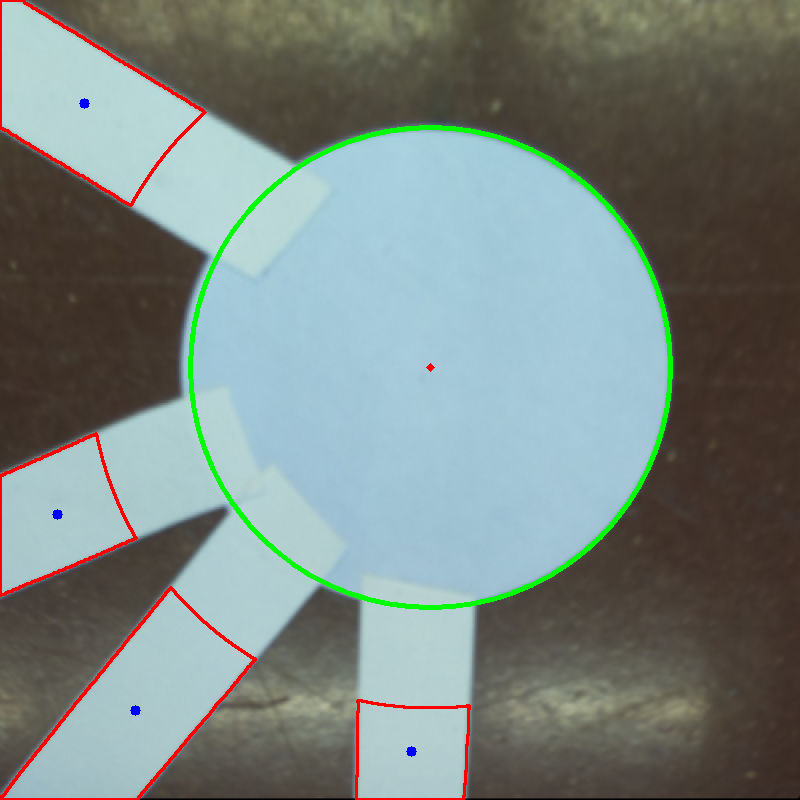
\includegraphics[width=0.95\linewidth]{assets/informatik-prototyp/opencv/angle_detection/edge_detect_centers.png} 
        \caption{Mittelpunkte der Kanten berechnen}
        \label{fig:edge-center}
        \end{subfigure}
        \begin{subfigure}{0.4\textwidth}
        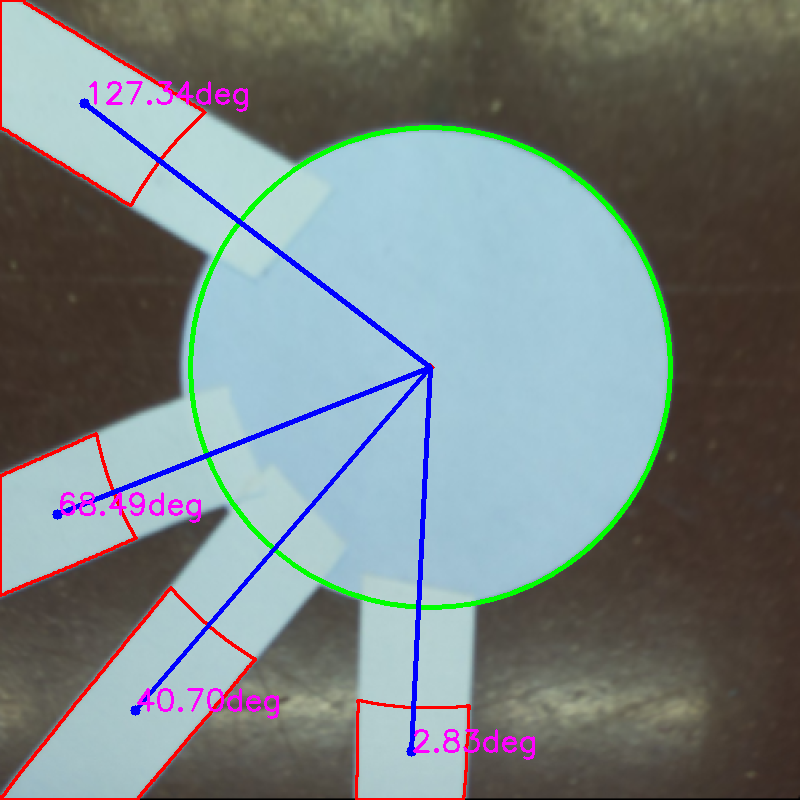
\includegraphics[width=0.95\linewidth]{assets/informatik-prototyp/opencv/angle_detection/node_with_edge_angles_annotated.png} 
        \caption{Winkel der Kanten}
        \label{fig:angle-lines}
        \end{subfigure}
        \caption{Winkel der einzelnen Kanten detektieren}
        \label{fig:node-with-edge-angles}
        \end{figure}
\end{enumerate}

\subsubsection{Graph-, Pylonen- und Barrierenerkennung}

% \textbf{Spiegelung}

% Starke Spiegelungen stellen ein grosses Problem bei der Erkennung von Knoten dar. Um die Bilder zu entspiegeln, können die Lichtverhältnisse angepasst, Polfilter verwendet oder Nachbearbeitungen durchgeführt werden.\cite{avoid-reflection}

% Beleuchtung

Als Basis fuer die Bilderkennung, wurde ein Graph aufgeklebt in der Mensa. Es wurden mehrere Bilder gemacht, wobei Pylonen und Barrieren willkuerlich auf Knoten und Kanten gestellt wurden und immer wieder verschoben wurden.

\textbf{OpenCV SIFT, FAST, ORB Algorithmen}

OpenCV bietet verschiedene Algorithmen zur Merkmalsdetektion und -beschreibung, die in der Bildverarbeitung und Computer Vision zum Objekterkennung und Tracking eingesetzt werden:

\begin{enumerate}
    \item SIFT (Scale-Invariant Feature Transform)
    
    SIFT ist ein Algorithmus, der robuste und skalierungsinvariante Merkmale in Bildern erkennt. Er findet markante Punkte, sogenannte Keypoints, und berechnet Deskriptoren, die invariant gegenüber Skalierung, Rotation und Beleuchtung sind. Es eignet sich gut für Objektwiedererkennung und Bildregistrierung.

    \item FAST (Features from Accelerated Segment Test)
    
    FAST ist ein sehr schneller Eckendetektor, der besonders für Echtzeitanwendungen geeignet ist. Er überprüft, ob ein Pixel ein Merkmal (Ecke) ist, indem es die Intensitäten der Pixel in einem kreisförmigen Muster um es herum vergleicht. Es ist jedoch nicht robust gegenüber Skalierung oder Rotation.

    \item ORB (Oriented FAST and Rotated BRIEF)
    
    ORB kombiniert FAST für die Merkmalsdetektion und BRIEF (Binary Robust Independent Elementary Features) für die Merkmalsbeschreibung. Es erweitert FAST, indem es Orientierung und Rotation berücksichtigt, und bietet eine effiziente, patentfreie Alternative zu SIFT und SURF, mit ähnlicher Genauigkeit und deutlich besserer Performance.
\end{enumerate}

Zusammenfassend:

\begin{itemize}
    \item SIFT ist genau und robust, aber rechenintensiv.
    \item FAST ist schnell, aber weniger robust.
    \item ORB ist ein guter Kompromiss zwischen Geschwindigkeit und Genauigkeit.
\end{itemize}

Aus unseren Test funktionieren alle diese Algorithmen sehr gut um zweidimensionale Objekte zu detektieren, wie nachfolgend an den Stickers auf der Notebook-Rückseite zu erkennen:

\begin{figure}[H]
    \centering
    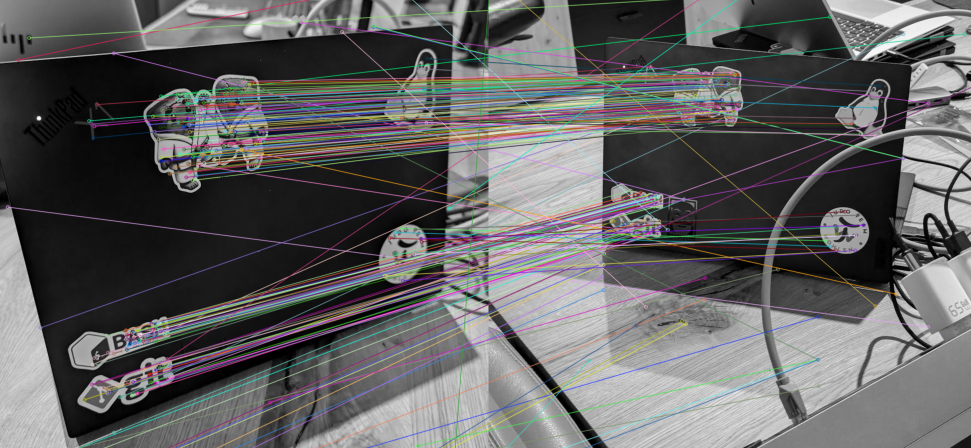
\includegraphics[width=1\linewidth]{assets/informatik-prototyp/opencv/sift/sift_good_example.png}
    \caption{Gutes Beispiel von SIFT Algorymtus}
    \label{fig:good-sift-example}
\end{figure}

Da unsere Objekte jedoch dreidimensionale sind und eine freie Rotation und Position in einem dredimensionalen Raum haben, ist es für den Algorithmus sehr schwierig Objektmerkmale festzulegen und diese in den verschiedenen Szenarien wieder zu detektieren:

\begin{figure}[H]
    \centering
\begin{subfigure}{1\textwidth}
    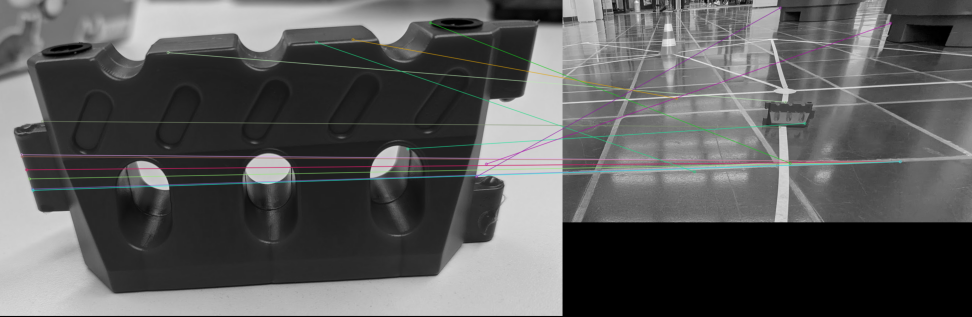
\includegraphics[width=1\linewidth]{assets/informatik-prototyp/opencv/sift/sift_our_usecase_example.png}
    \caption{SIFT Algorithmus}
    \label{fig:bad-sift-example}
\end{subfigure}
\begin{subfigure}{1\textwidth}
    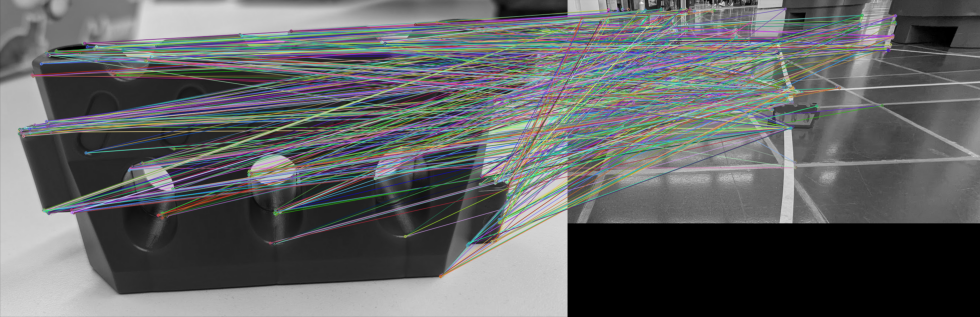
\includegraphics[width=1\linewidth]{assets/informatik-prototyp/opencv/sift/orb_our_usecase_example.png}
    \caption{ORB Algorithmus}
    \label{fig:bad-orb-example}
\end{subfigure}
    \caption{SIFT und ORB in unserem Usecase}
    \label{fig:sift-orb-in-our-usecase}
\end{figure}


Aus diesem Test Können wir entscheiden, dass die OpenCV Merkmalsdetektions Algorytmen nicht aussreichen, um Objekte in der 3D Umgebung sauber zu detektieren. Desshalb wird dieser Ansatz nicht mehr weiter verfolgt.

\textbf{Objekterkennung mit Farberkennung}

Grundsätzlich können Objekte auch nur rein durch ihre Farbe detektiert werden. Jedoch sind die Resultate stark von Umgebungsbedingungen abhängig.
Wir haben grundsätzlich 3 oder 4 verschieden Objekte zu detekieren:
\begin{itemize}
    \item Pylone (Orange)
    \item Barriere (Rot)
    \item Barriere (Weiss)
    \item Knoten (Weiss)
\end{itemize}

Orange und Rote Objekte können grundsätzlich sehr einfach detektiert werden. Da diese Farben in der Umgebung wo der Roboter schlussendlich operiert, sehr eindeutig sind:

\begin{figure}[H]
    \centering
    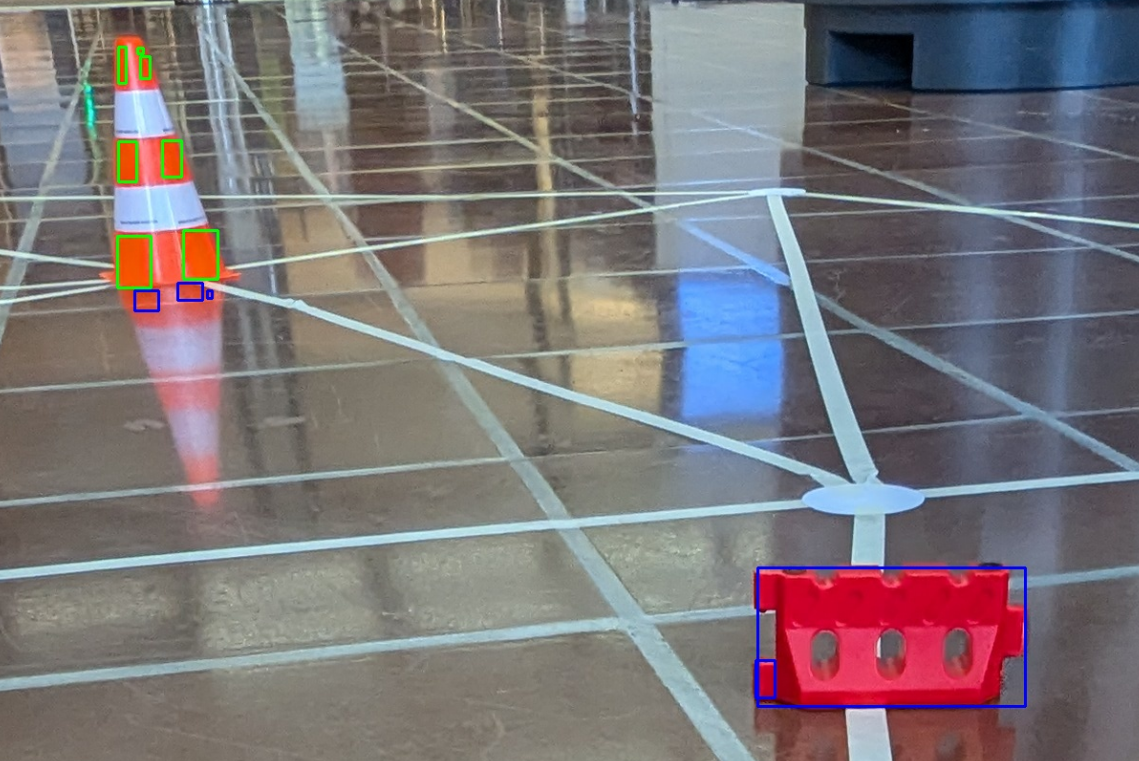
\includegraphics[width=1\linewidth]{assets/informatik-prototyp/opencv/object_detection_with_hsv/hsv_object_detection.png}
    \caption{Objekterkennung mittels Farberkennung der roten Barriere und orangen Pylone}
    \label{fig:opencv_hsv_object_detection_good}
\end{figure}


Die weisse Barriere und der weisse Knoten macht es jedoch schwieriger, denn einerseits haben sie die gleiche Farbe, was das unterscheiden dieser schwierig macht, und unter anderem haben wir, unter verschiedenen Lichtverhältnissen, Spiegelungen, welche sich im bild auch als weisse Flecken darstellen:

\begin{figure}[H]
    \centering
    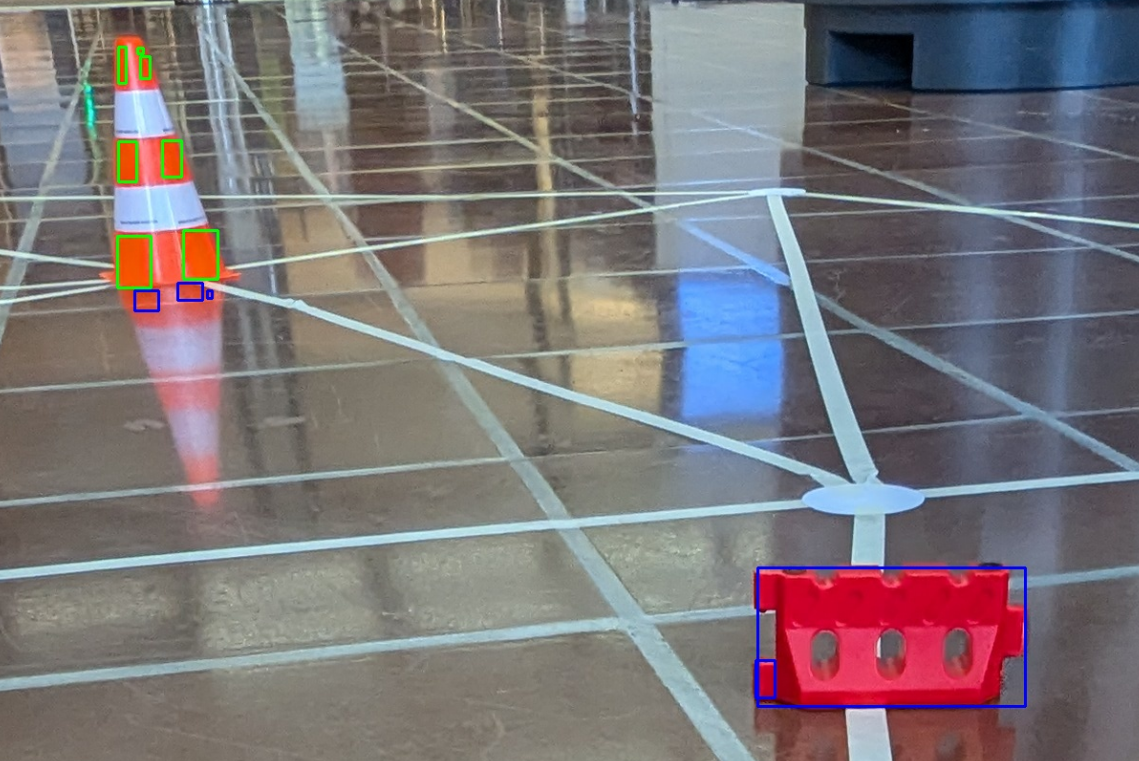
\includegraphics[width=1\linewidth]{assets/informatik-prototyp/opencv/object_detection_with_hsv/hsv_object_detection.png}
    \caption{Objekterkennung mittels Farberkennung der roten Barriere und orangen Pylone}
    \label{fig:opencv_hsv_object_detection_good}
\end{figure}


\begin{itemize}
    \item Beleuchtung: Änderungen im Licht können die Farbgenauigkeit beeinflussen.
    \item Hintergrund: Farben im Hintergrund können zu Fehlklassifikationen führen.
    \item Kalibrierung: Bestimme die Farbbereiche (lower, upper) individuell für die Umgebung.
    \item Performance: Farbmasken können effizient auf Echtzeitanwendungen angewendet werden.
\end{itemize}

\textbf{Vorteile:}
\begin{itemize}
    \item Einfach und schnell: Geringe Rechenleistung erforderlich.
    \item Intuitiv: Keine komplexen Modelle notwendig.
    \item Robust für klare Farben: Funktioniert gut, wenn die Farben eindeutig sind.
\end{itemize}
\textbf{Nachteile:}
\begin{itemize}
    \item Empfindlichkeit gegenüber Licht: Variierende Beleuchtung beeinträchtigt die Erkennung.
    \item Begrenzte Flexibilität: Funktioniert schlecht bei ähnlichen Farben oder gemusterten Objekten.
    \item Störanfälligkeit: Hintergrundrauschen kann Probleme bereiten.
\end{itemize}


Die Objekterkennung von OpenCV kann die Hindernisse recht sicher erkennen, jedoch ist es nicht moeglich die Knoten zu detektieren.

\textbf{YOLOv11}

Auf Roboflow\footnote{https://roboflow.com/} wurden die insgesamt 58 erstellten Bilder labeled.
Das bedeutet, dass manuell die zu erkennenden Objekte ausgewaehlt und zu bestimmten Klassen hinzugefuegt wurden.

Danach wird das Datenset unterteilt in verschiedene Gruppen: Train, Validation, Test. Die Training Daten werden verwendet mit den Markierungen, damit das Model davon lernen kann. Das Validierungsset wird benoetigt, um waehrend dem Trainingsprozess zu pruefen, wie gut das Model ist und wie es angepasst werden soll. Das Testset wird schlussendlich verwendet, um zu testen, wie gut das angepasste Model die einzelnen Elemente erkennt. Dieses Testset ist noetig, weil es wichtig ist, dass die Daten, die schlussendlich verwendet werden, um zu pruefen, wie gut das Model ist, dem Model noch komplett unbekannt sein sollten.
\begin{figure}[H]
    \centering
    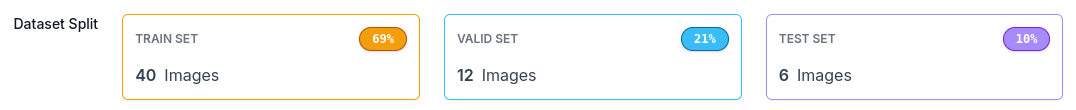
\includegraphics[width=\linewidth]{assets/informatik-prototyp/yolo/dataset-split.png}
    \caption{Datenset Split}
    \label{fig:data-split}
\end{figure}

Als erstes wurden versucht ein Model zu trainieren, das alle Graphenelemente (Knoten und Kanten) und Hindernisse erkennt:

\begin{figure}[H]
\begin{subfigure}{0.55\textwidth}
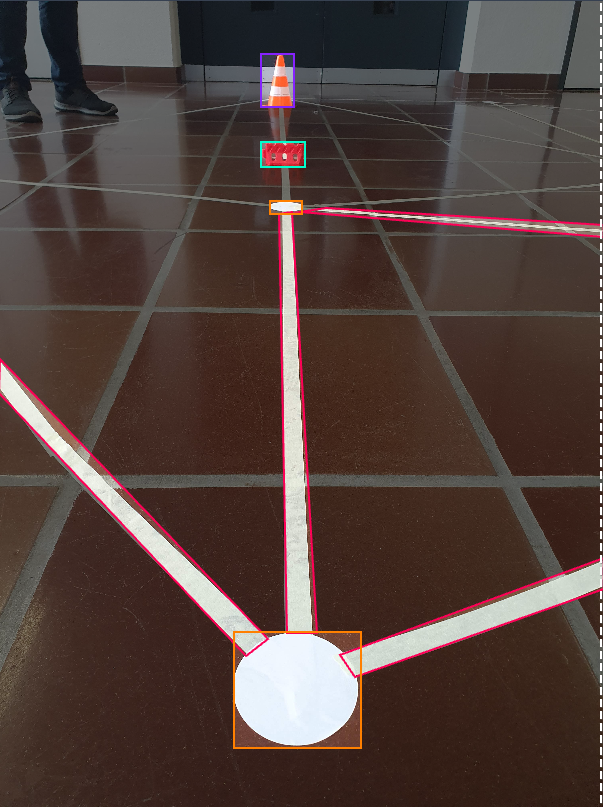
\includegraphics[width=0.95\linewidth]{assets/informatik-prototyp/yolo/labeled-image-lines.png} 
\caption{Bild mit Elementen + Linie markiert}
\label{fig:labeled-image-lines}
\end{subfigure}
\begin{subfigure}{0.4\textwidth}
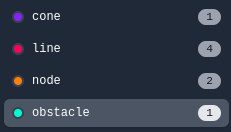
\includegraphics[width=0.95\linewidth]{assets/informatik-prototyp/yolo/labeled-classes-lines.png} 
\caption{Markierte Klassen mit Linie}
\label{fig:line-classes-lines}
\end{subfigure}

\caption{Roboflow labeled Bild mit Linien}
\label{fig:labeling-with-lines}
\end{figure}


Mihilfe eines Jupyter Notebooks, das von Roboflow zur Verfuegung gestellt wird, wurde ein YOLO Model mit 10 Epochs\footnote{https://deepai.org/machine-learning-glossary-and-terms/epoch} trainiert. Danach wurden Bilder aus dem Testset genutzt, wobei das Model versucht die einzelnen Elemente zu erkennen. Zusaetzlich wurde eine Confusion Matrix\footnote{https://www.sciencedirect.com/topics/engineering/confusion-matrix\#:\~:text=A\%20confusion\%20matrix\%20represents\%20the,by\%20model\%20as\%20other\%20class.} erstellt, die zeigt, welche Elemente als was erkannt wurde.

\begin{figure}[H]
\begin{subfigure}{0.3\textwidth}
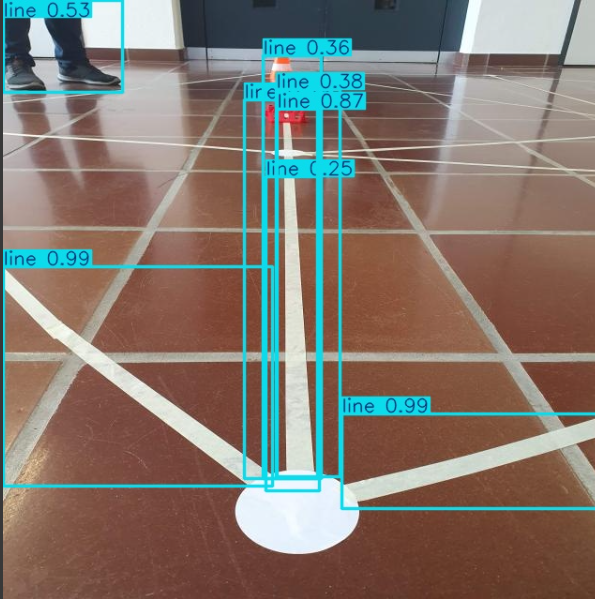
\includegraphics[width=0.95\linewidth]{assets/informatik-prototyp/yolo/line-recognitions.png} 
\caption{Erkanntes Bild mit Linien}
\label{fig:image-recognition-with-lines}
\end{subfigure}
\begin{subfigure}{0.69\textwidth}
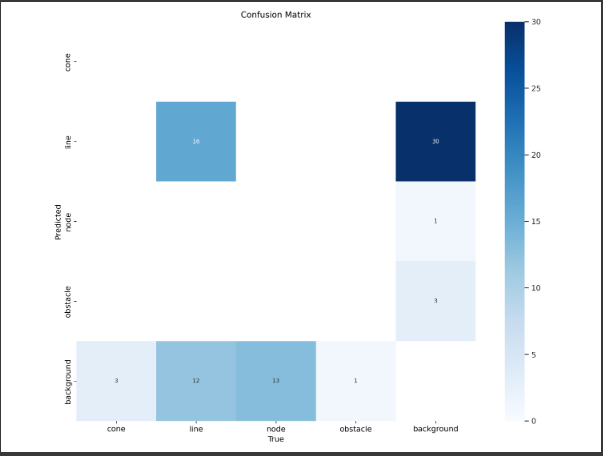
\includegraphics[width=0.95\linewidth]{assets/informatik-prototyp/yolo/conf-matrix-lines.png} 
\caption{Confusion Matrix mit Linien}
\label{fig:conf-matrix-lines}
\end{subfigure}

\caption{Bilderkennung inklusive Linien}
\label{fig:recognition-with-lines}
\end{figure}

Aus diesem Experiment war klar, sowohl aus dem Bild mit den "erkannten" Linien, als auch von der Confusion Matrix, dass Linien nicht korrekt erkannt werden koennen.
Aus der Confusion Matrix kann gelesen werden, dass von allen erkannten Linien in 4 Bildern, 30 Linien erkannt wurden an Stellen, an denen sich gar nichts befindet ("background").

Als naechste wurde das gleiche noch einmal durchgefuehrt. Dieses Mal wurde die Line-Klasse entfernt und es wurden nur noch Knoten, Pylonen und Barrieren markiert.

\begin{figure}[H]
\begin{subfigure}{0.55\textwidth}
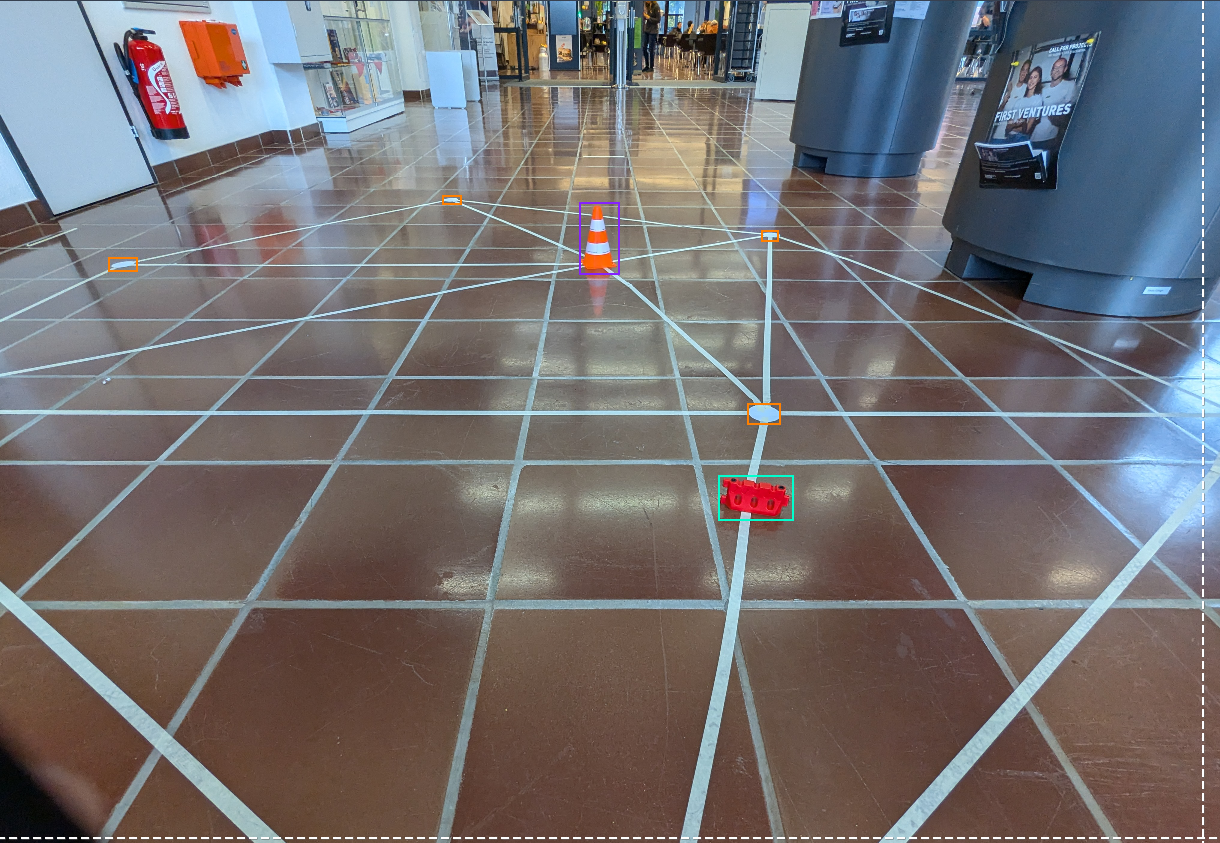
\includegraphics[width=0.95\linewidth]{assets/informatik-prototyp/yolo/labeled-image.png} 
\caption{Bild mit Elementen markiert}
\label{fig:labeled-image}
\end{subfigure}
\begin{subfigure}{0.4\textwidth}
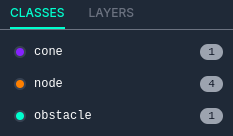
\includegraphics[width=0.95\linewidth]{assets/informatik-prototyp/yolo/labeled-classes.png} 
\caption{Markierte Klassen}
\label{fig:line-classes}
\end{subfigure}

\caption{Roboflow labeled Bild mit Linien}
\label{fig:labeling-with-lines}
\end{figure}

Die Bilderkennung des selben Jupyter Notebooks mit den reduzierten Klassen sah wie folgt aus:

\begin{figure}[H]
\centering
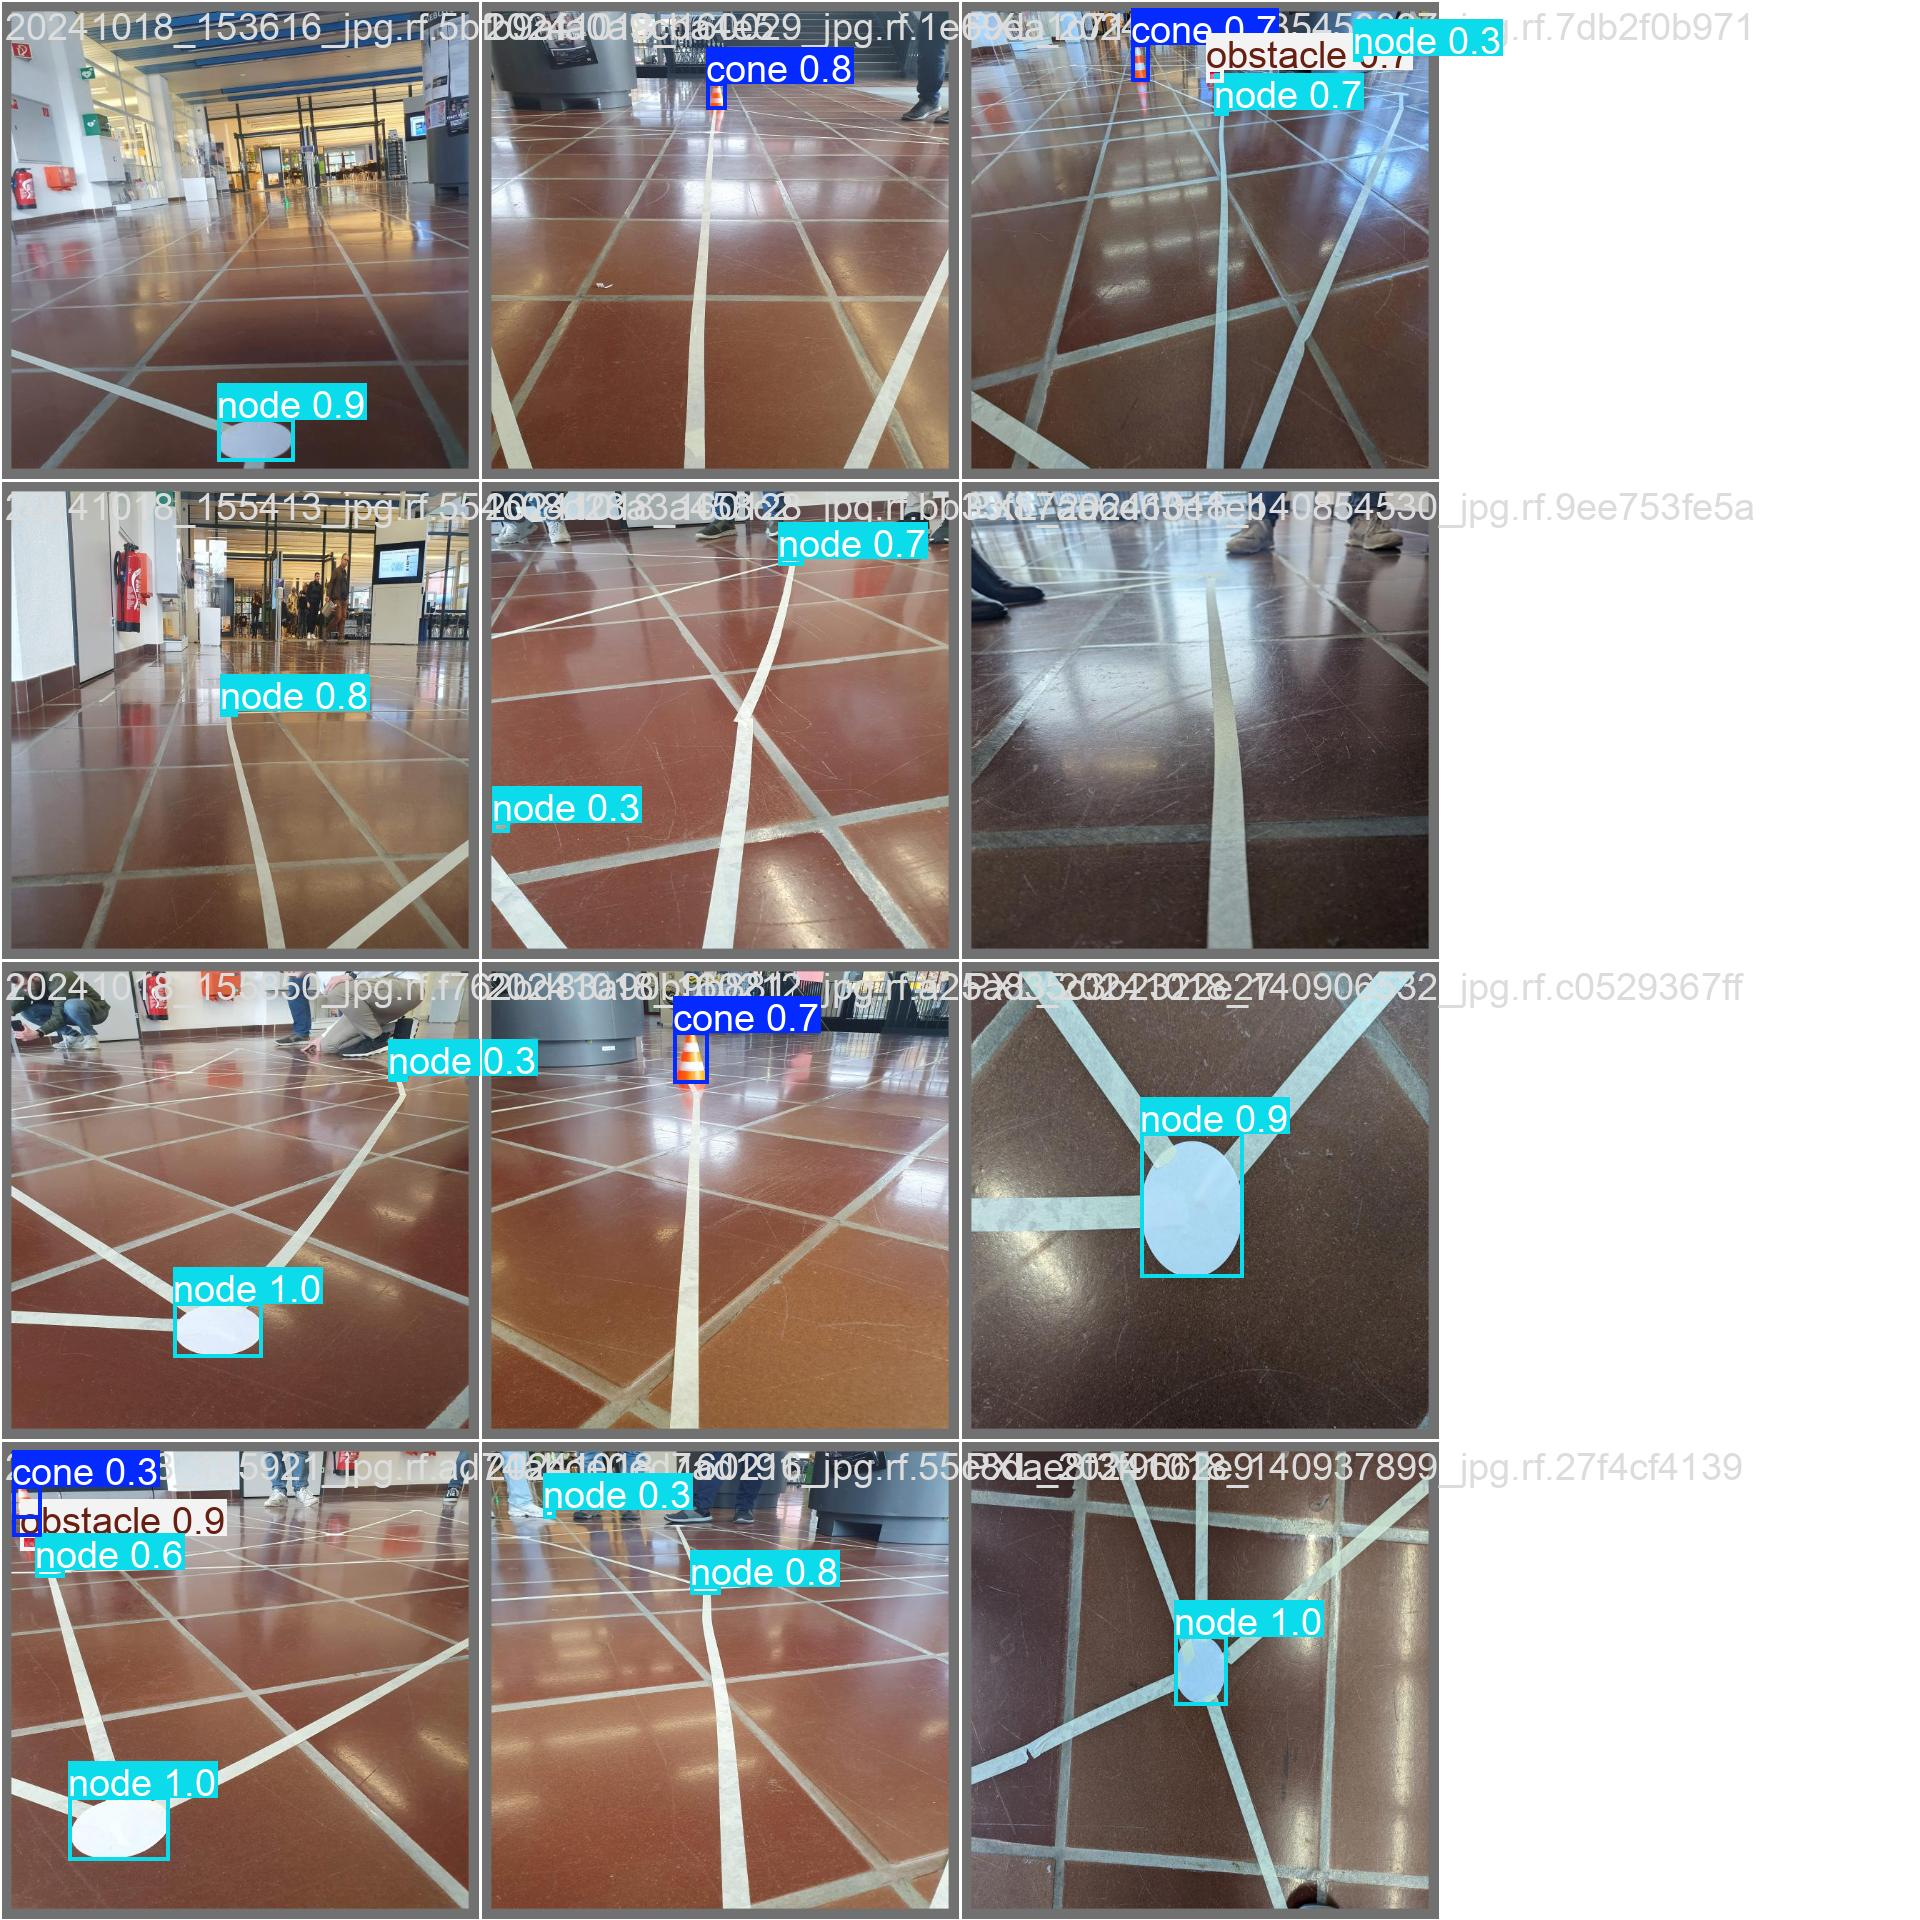
\includegraphics[width=\textwidth -30mm]{assets/informatik-prototyp/yolo/recognized-images.jpeg}
\caption{YOLOv11 Bilderkennung}
\label{fig:img-recognition-yolo}
\end{figure}

\begin{figure}[H]
\centering
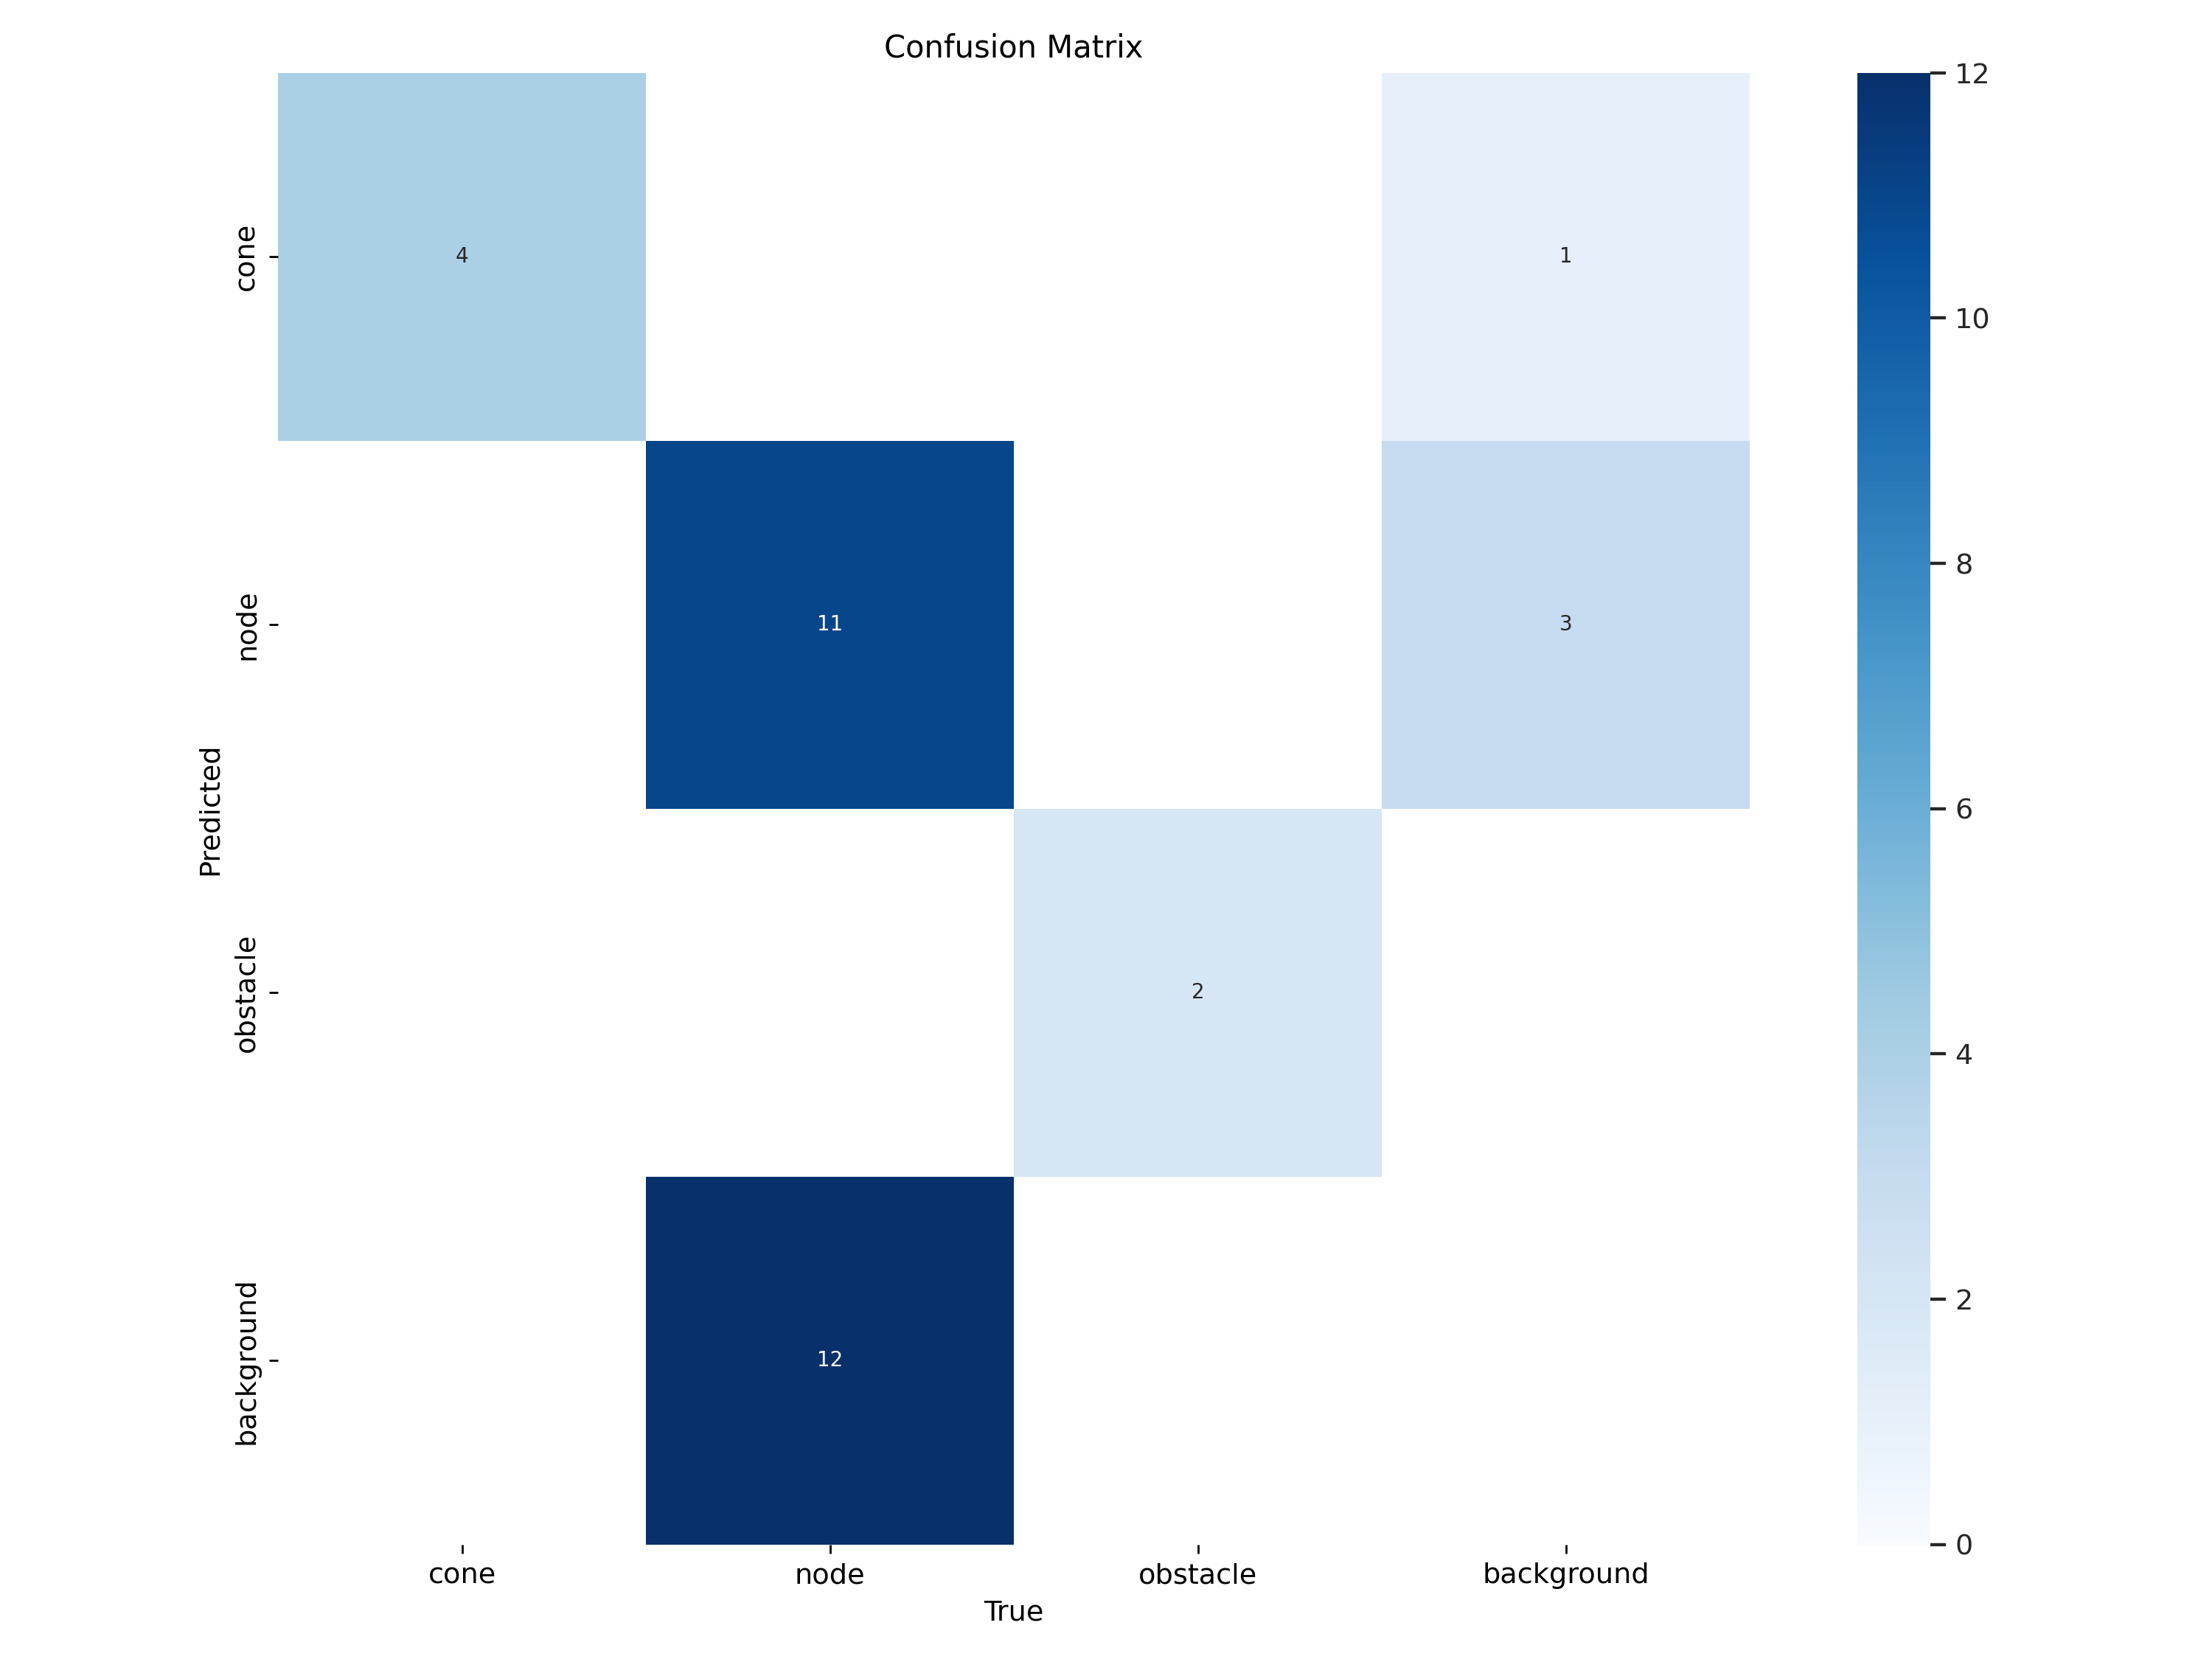
\includegraphics[width=\textwidth -20mm]{assets/informatik-prototyp/yolo/conf-matrix.png}
\caption{YOLOv11 Confusion Matrix Knoten, Barrieren und Pylonen}
\label{fig:conf-matrix-yolo}
\end{figure}

Aus dieser Matrix kann gelesen werden, dass alle Pylonen und alle Barrieren richtig erkannt werden. Einmal wird eine Pylone erkannt, obwohl es keine gibt. Die meisten vorausgesagten Knoten, sind wirklich Knoten, jedoch werden viele Knoten nicht erkannt. Dabei muss jedoch bedacht werden, dass es einfacher ist fuer das Model Knoten zu erkennen, die nahe und dadurch deutlicher sind und dass das Trainingsdatenset sehr klein ist. Trotzdem besteht ein sehr wahrscheinliches Risiko, dass ein Knoten nicht erkannt werden koennte.

Das gleiche Experiment wurde noch einmal durchgefuehrt mit nur Pylonen und Barrieren:

\begin{figure}[H]
\begin{subfigure}{0.55\textwidth}
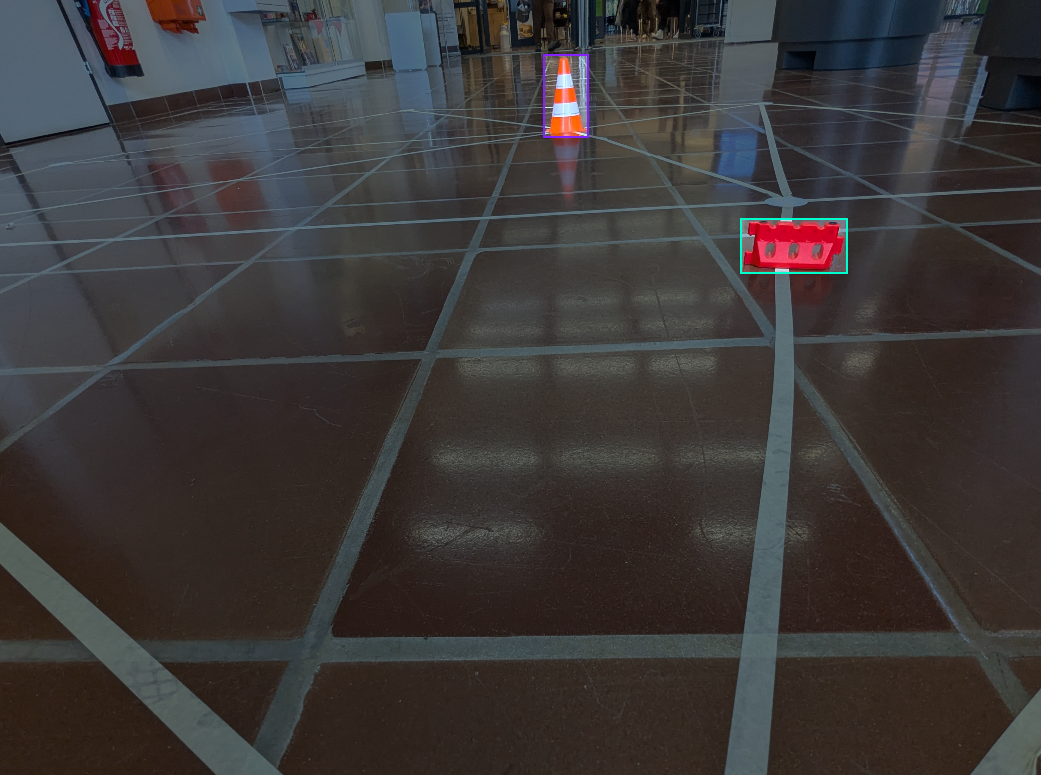
\includegraphics[width=0.95\linewidth]{assets/informatik-prototyp/yolo/label-cone-obstacle.png} 
\caption{Bild mit Hindernissen markiert}
\label{fig:labeled-image-obst}
\end{subfigure}
\begin{subfigure}{0.4\textwidth}
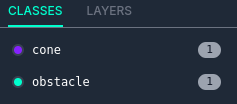
\includegraphics[width=0.95\linewidth]{assets/informatik-prototyp/yolo/classes-cone-obstacle.png} 
\caption{Markierte Klassen}
\label{fig:cone-obst-classes}
\end{subfigure}
\caption{Roboflow labeled Bild nur mit Hindernissen}
\label{fig:labeling-with-cone-obst}
\end{figure}


Die Resultate fuer die Pylonen und die Barrieren ist dasselbe, wie im vorherigen Experiment, jedoch faellt, wie erwartet die Unsicherheit der Knoten weg. Das Problem ist es nun, dass aus den erkannten Elementen auf dem dargestellten Bild geschlossen werden wuerde, dass sich auf dem naechsten Knoten ein Pylon befindet, da der vorherige Knoten nicht mehr erkannt wird.

\begin{figure}[H]
\begin{subfigure}{0.5\textwidth}
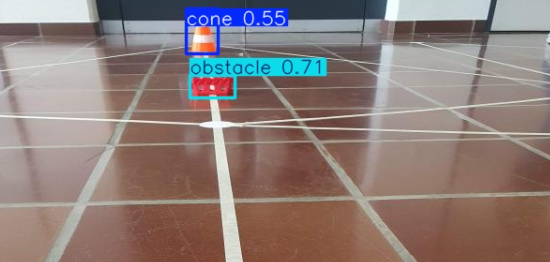
\includegraphics[width=0.95\linewidth]{assets/informatik-prototyp/yolo/cone-obst-recognition.png} 
\caption{Erkanntes Bild mit Hindernissen}
\label{fig:image-recognition-with-cone-obst}
\end{subfigure}
\begin{subfigure}{0.5\textwidth}
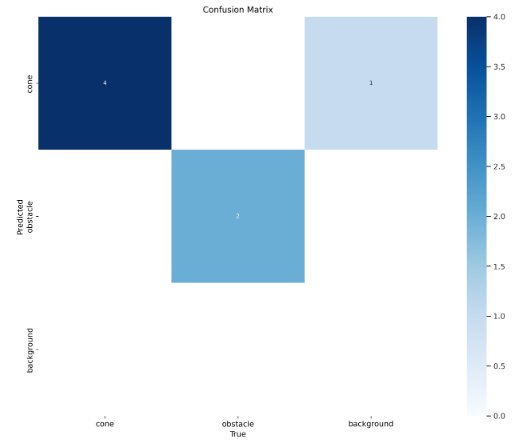
\includegraphics[width=0.95\linewidth]{assets/informatik-prototyp/yolo/cone-obst-conf-matrix.png} 
\caption{Confusion Matrix mit Hindernissen}
\label{fig:conf-matrix-cone-obst}
\end{subfigure}

\caption{Bilderkennung mit Hindernissen}
\label{fig:recognition-with-cone-obst}
\end{figure}



\textbf{Fazit}

Zur Erkennung der Hindernisse und des Graphens, funktionierte YOLO am besten. Dabei wird versucht werden die Hindernisse und die Graphenknoten zu erkennen. Die Unsicherheit der Knotenerkennung ist ein grosses Risiko. Deshalb wird versucht eine Strategie zu finden, die mit den ausgehenden Linien vom Knoten arbeitet und wobei nur die jeweils naechsten Knoten erkannt werden muessen.